\documentclass[9pt,a4paper,twocolumn,twoside]{tau-class/tau}

\usepackage{listings}

\lstset{
    language=C++,
}

\title{Design and Build a Balancing Robot}

\author{Name\thanks{email@anu.edu.au}}

\affil[1]{Research School of Physics, Australian National University, Canberra ACT, 2601, Australia}

\begin{abstract}
\end{abstract}

\begin{document}

\maketitle

\section{Executive Summary}
Executive Summary

\section{Introduction}
\subsection{Background}
Background

\subsection{Requirements Review}
\label{subsec:requirements_review}
The primary objective of this project is to build an autonomous self-balancing robot which is able to move to or keep itself around a designated position. To achieve this, the listed specific requirements are as follows:
\begin{itemize}
	\item Top-level requirements: \begin{itemize}
	\item The robot must maintain its balanced position without any falling cases.
	\item If the robot is perturbed externally (e.g., a deliberated push, or an obstacle collided), it must be able to return balanced within $2s$. The perturbation is defined as changing its pitch angle up to $15^\circ$.
	\item Without perturbation, the robot must balance itself in a small range. It must not move more than $0.5m$ in $1s$.
	\end{itemize}

	\item Electronic components:\begin{itemize}
	\item The robot must be able to sense its angle or velocity at $>10Hz$. The resolution of angle must be $<0.5^\circ$.
	\item The robot must take action within $0.1s$ after a controlling signal is sent.
	\item The electronics must be stable during its runtime.
	\item After turning on,  the robot must work entirely independently, including power supply, signal processing, and controlling.
	\end{itemize}

	\item Physical structure:\begin{itemize}
	\item The structure must be stable enough that the position of mass center doesn't change.
	\item The chassis must be sturdy, which can resist damage when the robot falls in some cases.
	\end{itemize}
  
  \item Advanced requirements: \begin{itemize}
  \item The robot can be able to fully control its state, including facing direction and moving speed.
  \item The robot can follow a designated path without obvious drift.
  \item The robot can smartly respond to different situations: in peaceful environments, being slightly perturbed, being strongly perturbed, set to move to and keep around a position. 
  \end{itemize}
\end{itemize}


\section{Technical Details and Analysis}

\subsection{Basic Ideas}
\label{subsec:basic_ideas}

\figref{fig:basic_balancing_flowchart} shows the flowchart of the basic balancing idea of the robot. Generally, it shows the realization of the basic balancing skills. Any other advanced skills can be add to these parts. Reading multiple types of states (e.g., pitch angle, yaw angle, and x-acceleration) can be add in the "Read State" process. "Check States" decision can be used to assess the situation of the robot. "Feedback Controller" process can handle different controllers, such as PID controller. "Take Action" process controls the states of the robot.

\begin{figure}[htbp]
    \centering
    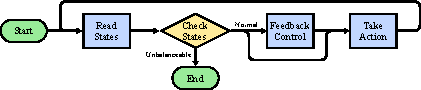
\includegraphics[width=\columnwidth]{figures/basic_balancing.pdf}
    \caption{Flowchart of basic balancing logic. After turning on, the robot keeps reading its state, such as the pitch angle or the angular velocity of y-axis. If it's not strongly unbalanced, feedback controllers are used to generate an output from the state. The output is used to control the robot, such as moving forward or turn left. The feedback loop can balance the robot theoretically.}
    \label{fig:basic_balancing_flowchart}
\end{figure}

We started from developing the basic balancing skill. When this first stage was completed successfully, we would try to realize the advanced requirements by upgrading the existed processes or decisions instead of rebuild a new structure. In this way, the development would be controllable and the progress would be clear. However, a new structure can be required if we want to develop a more complex logic.

% \begin{lstlisting}[caption={Main logical code in Arduino IDE.}, label={lst:arduino_logic_code},language=C++]
% void setup() {
%   Serial.begin(115200);
%   setupSuccess &= connectImu();
%   setupSuccess &= connectPID();
%   setupSuccess &= connectMotor();
%   Serial.print(F("Setup succeed: "));
%   Serial.println(setupSuccess);
% }

% void loop() {
%   if (!setupSuccess) { return; }
%   if (!imuHasData) { return; }
%   if (!getImuAngle()) { return; }
%   getMotorValue();
%   driveMotor();
% }
% \end{lstlisting}

\subsection{Electronic Components}
To achieve the main goal, the electronic components should contain these necessary parts: a state sensor, a central processor, an action driver, and power supply.

\subsubsection{The state sensor}
We use MPU-6050 inertial measurement unit (IMU) as the state sensor. It consists of a triple-axis gyroscope and a triple-axis accelerometer. Using the angular velocities and linear accelerations, we can get or calculate most of the important states of robot. The key parameters of MPU-6050 are listed in \tabref{tab:mpu6050_specifications}:

\begin{table}[htbp]
    \centering
    \begin{tabular}{c c c}
    \toprule
    \textbf{Parameter} & \textbf{Value} & \textbf{Unit} \\
    \midrule
    Gyroscope Full-scale Range & $\pm250$ & $^\circ/s$\\
    Gyroscope Sensitivity & $131$ & $LSB/(^\circ/s)$\\
    Gyroscope Noise Spectral Density & $0.005$ & $^\circ/s/\sqrt{Hz}$\\
    Gyroscope Output Rate & $8000$ & $Hz$\\
    \midrule
    Accelerometer Full-scale Range & $\pm2$ & $g$\\
    Accelerometer Sensitivity & $16384$ & $LSB/g$\\
    Accelerometer Noise Spectral Density & $400$ & $\mu g/\sqrt{Hz}$\\
    Accelerometer Output Rate & $1000$ & $Hz$\\
    \midrule
    Supported Communication & $I^2C$ & \\
    Communication Speed & $400$ & $kHz$ \\
    Clocking Speed & $32.768k\sim19.2M$ & $Hz$ \\
    \midrule
    Power Input Voltage & $2.375\sim3.46$ & $V$ \\
    \bottomrule
    \end{tabular}
    \vspace{\baselineskip}
    \caption{The key parameters of MPU-6050 inertial measurement unit \cite{mpu6050_datasheet}}
    \label{tab:mpu6050_specifications}
\end{table}

The best resolution of angular velocity can reach $7.6\times10^{-3}\;^\circ/s$, and the best resolution of acceleration can reach $61\times10^{-6}\;g$. Ignoring the noise, these resolutions are totally sufficient for the requirements. Both the sampling rate and communication speed satisfy our requirements. The only disadvantage is the sensor noise or drift. Considering the noise, we can try to process the signal (such as low-pass filter or quaternion) to get high enough resolution. 

\subsubsection{The central processor}
Arduino UNO is chosen as the processor. We can use it to get data from the IMU, process the data, and control the action driver. Its key parameters are listed in \tabref{tab:arduino_uno_specifications}:

\begin{table}[htbp]
    \centering
    \begin{tabular}{c c c}
    \toprule
    \textbf{Parameter} & \textbf{Value} & \textbf{Unit} \\
    \midrule
    \# Digital I/O Pins & $14$ & \\
    \# Analog Input Pins & $6$ & \\
    \# PWM Pins & $6$ & \\
    \midrule
    Supported Communication & $I^2C$, $SPI$, $UART$ & \\
    Clocking Speed & $16$ & $MHz$ \\
    \midrule
    Power Output Voltage & $3.3$, $5$ & $V$ \\
    Power Input Voltage & $7\sim12$ & $V$ \\
    \bottomrule
    \end{tabular}
    \vspace{\baselineskip}
    \caption{The key parameters of Arduino UNO \cite{arduino_uno_datasheet}}
    \label{tab:arduino_uno_specifications}
\end{table}

The number of digital, analog and PWM pins are enough for the wiring connecting the processor to the sensor and the action driver. The high processing speed is ideal for our control logic. Using $I^2C$ communication and $3V3$ output power, it can math the MPU-6050 very well. However, the power output voltage may not enough for some action drivers. So a shared power supply may be required. 

\subsubsection{The action driver}
We choose to use a L298N motor driver and two geared DC motors. The key parameters of the L298N motor driver are listed in \tabref{tab:l298n_specifications}:

\begin{table}[htbp]
    \centering
    \begin{tabular}{c c c}
    \toprule
    \textbf{Parameter} & \textbf{Value} & \textbf{Unit} \\
    \midrule
    Digital Input Pins & $IN1+IN2$, $IN3+IN4$ & \\
    PWM Input Pins & $ENA$, $ENB$ & \\
    \midrule
    Logic Input Voltage & $5$ & $V$ \\
    Power Output Voltage & $3.2\sim40$ & $V$ \\
    Power Input Voltage & $5\sim35$ & $V$ \\
    \bottomrule
    \end{tabular}
    \vspace{\baselineskip}
    \caption{The key parameters of L298N motor driver \cite{l298n_datasheet}}
    \label{tab:l298n_specifications}
\end{table}

The motor driver allows PWM input, which matches well with the Arduino UNO. The digital input pins can be used to control the direction of motors, while the PWM input pins can be used to control the speed. The required voltage is high as expected, so a good power supply is needed. However, by experiments, we found that the motors can keep still when the speed signal is small, which is likely caused by the resistance. Moreover, the two motors have a little asymmetry, which makes the robot yaw. Therefore, stepper motors can be required when we need to do precise control or measurement.

\subsubsection{Power supply}
We need to supply power to both the Arduino UNO and the motor driver. Therefore, two 800mAh 3.7V rechargeable Li-ion cells are used. For reusability, we use a breadboard to transfer the power from batteries to the two components instead of soldering the wires. The safe charged voltage of Li-ion is $2.8\sim4.2\;V$. By testing, the batteries need to be recharged after working for about 10 hours. 

\subsubsection{Wiring structure}
As mentioned above, the electronic components used are: 
\begin{itemize}
  \item MPU-6050 IMU
  \item Arduino UNO
  \item L298N motor driver
  \item Geared DC motors
  \item Li-ion Batteries
  \item Breadboard
\end{itemize}
The wiring method is shown in \figref{fig:wire_diagram}.

\begin{figure}[htbp]
    \centering
    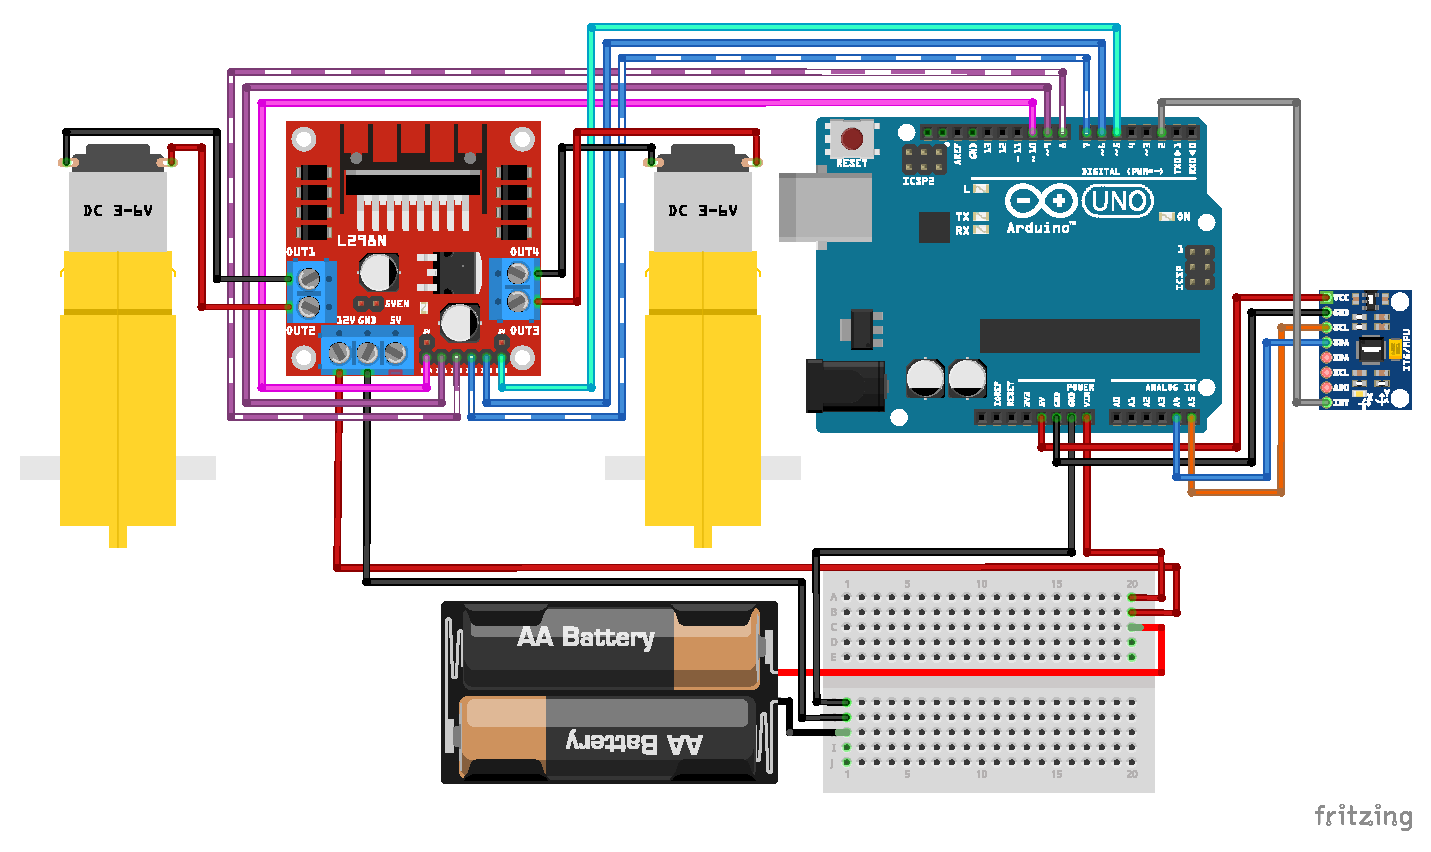
\includegraphics[width=\columnwidth]{figures/wire_diagram.pdf}
    \caption{Wiring diagram of the electronic components. The battery and breadboard are used to power the Arduino UNO and L298N motor driver. UNO communicates with MPU-6050 inertial measurement unit (IMU) using I2C protocol, and sends analog signal to the motor driver using pulse width modulation (PWM). The motor driver controls 2 motors.}
    \label{fig:wire_diagram}
\end{figure}

\subsection{Mechanical Design}

\subsubsection{Physical model analysis}
\figref{fig:physical_model} shows the simplified physical model of the robot. We can use Lagrangian mechanics to analyze the relationship between $F$ and $\theta$, $x$. The system Lagrangian and Euler–Lagrange equations are given by:
\begin{equation}
	L=\frac{1}{2}M\dot{x}^2+\frac{1}{2}m\left[(\dot{x}+l\dot{\theta}\cos{\theta})^2+(l\dot{\theta}\sin{\theta})^2\right]-mgl\cos{\theta}
\end{equation}

\begin{align}
	\frac{d}{dt}\frac{\partial L}{\partial\dot{x}}-\frac{\partial L}{\partial x}=F\quad&\Longrightarrow\quad(M+m)\ddot{x}+ml\ddot{\theta}\cos{\theta}-ml\dot{\theta}^2\sin{\theta}=F\label{eq:el_eq1}\\
	\frac{d}{dt}\frac{\partial L}{\partial\dot{\theta}}-\frac{\partial L}{\partial\theta}=0\quad&\Longrightarrow\quad \ddot{x}\cos{\theta}+l\ddot{\theta}-g\sin{\theta}=0\label{eq:el_eq2}
\end{align}

\begin{figure}[htbp]
    \centering
    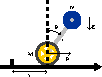
\includegraphics[width=0.6\columnwidth]{figures/physical_model.pdf}
    \caption{A simplified physical model of the robot. Constrain the movement in 1 dimension. THe model consists of a wheel with mass $M$, a body mass center $m$, and a light stick connecting these two with length $l$. The action of wheel is simplified as a force $F$. Assume the robot is at position $x$ and its pitch angle is $\theta$.}
    \label{fig:physical_model}
\end{figure}

Usually, we care about the dynamic of $\theta$, which can be derived from \equref{eq:el_eq1} and \equref{eq:el_eq2}:

\begin{equation}
	\ddot{\theta}=\frac{(M+m)g\sin{\theta}-F\cos{\theta}}{(M+m\sin^2{\theta})l}-\frac{m\dot{\theta}^2\sin{2\theta}}{2(M+m\sin^2{\theta})}
    \label{eq:theta_dynamic}
\end{equation}

According to the model \figref{fig:physical_model} and this \equref{eq:theta_dynamic}, we can analyze some cases:
\begin{itemize}
	\item The robot is perfectly at the balanced state, but a perturbation happens before the controller realizes it (i.e., $\theta\gtrapprox0$, $F=\dot{\theta}=0$). In this case, $\ddot{\theta}\approx\frac{(M+m)g\sin{\theta}}{lM}$. To save time for the controller to realize before $\theta$ becomes too large, we want $\ddot{\theta}$ to be as small as possible, which means we need to use small $m$ and/or large $l$.
	\item The robot is at an unbalanced but stable state (i.e., $\theta>0$, $\ddot{\theta}\approx\dot{\theta}\approx0$). To keep a constant $\theta$, it's necessary to make $F=(M+m)g\tan{\theta}$. However, because of the limit of motor power, $F$ can be maintained for only a short time before the large speed brings large resistance. So we should make $F>(M+m)g\tan{\theta}$ to bring back balance before the saturation of motors.
	\item The robot is severely unbalanced (i.e., $\theta>0$, $\dot{\theta}>0$). In this case, the only possible way to balance the robot is to make $\ddot{\theta}$ as negative as possible (i.e., $\ddot{\theta}\ll0$). To achieve this, we need to use a combination of large $F>(M+m)g\tan{\theta}$ and small $l$.
	\item The robot is inverted (i.e., $90^\circ<\theta<270^\circ$ ($l<R_\text{wheel}$), $l=0$, or $m=0$). Now the robot is impossible to return to the desired balanced state (or the balanced state can't be defined), but becomes permanently stable.
\end{itemize}
In conclusion, a motor being able to produce huge $F$ is wanted for all the cases. Similarly, it's good to have small $m$, $M$, and/or $\frac{m}{M}$. Large $l$ is suitable for peaceful environment and high balance performance, while small $l$ or inverted robot is suitable for severe environment and high controllability. 

\subsubsection{Chassis}
We use CAD (Autodesk Fusion) to design the chassis model, and 3D-print the model. The chassis is designed with many components in the experimental stage to make some components easier to update. These components are assembled using M3 bolts and nuts. For the final design, all the components are combined into a whole one to make the chassis stable.

In Fusion, the chassis is designed with the help of the models of other electronic components. Official datasheets of the electronic components are also used. In this way, it's precise and accurate to design the size and position of chassis components and through holes. One of our CAD model designs is shown in \figref{fig:chassis_design}. It has high mass center, which can perform good balancing skill but lack controllability.
\begin{figure}[htbp]
  \centering
  \begin{subfigure}{0.8\columnwidth}
    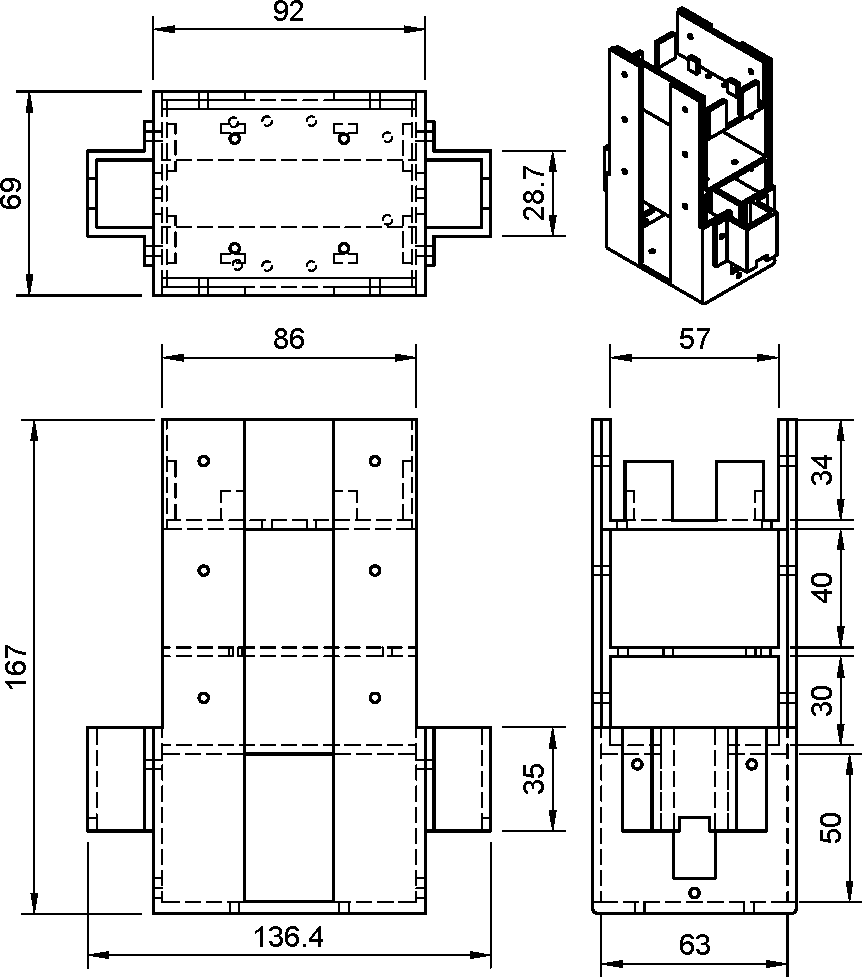
\includegraphics[width=\linewidth]{figures/front_top_side.pdf}
    \caption{Front-top-side view}
  \end{subfigure}

  \vspace{\baselineskip}

  \begin{subfigure}{0.8\columnwidth}
    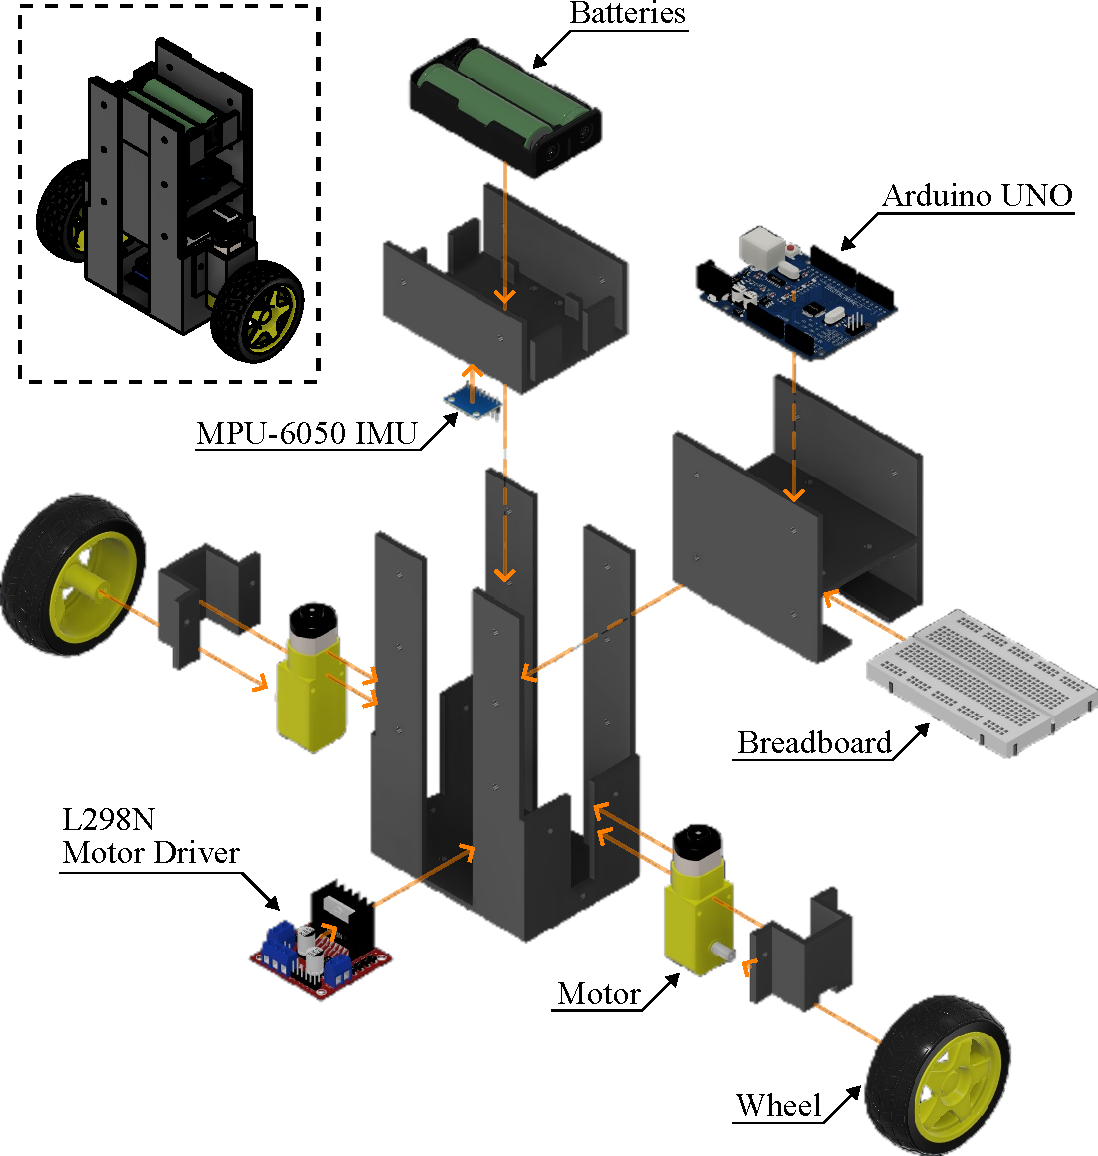
\includegraphics[width=\linewidth]{figures/assembly_manual.pdf}
    \caption{Robot components and assembly}
  \end{subfigure}
  \caption{A chassis model design.}
  \label{fig:chassis_design}
\end{figure}

PrusaSlicer is used to convert CAD models to 3D-printing code. The printer uses PLA as the filament with diameter of $1.75mm$. To make our chassis sturdy, we use layer height of $0.3mm$. The vertical shells is set to 4 perimeters, and the horizontal shells is set to 4 top layers and 4 bottom layers. Since most of our chassis consist of plates of $3mm$, these parameters are sufficient to make our chassis solid. The fill density is set to $15\%$. The only disadvantage is that solid chassis may increase the mass. We compensated it by change the height of mass center by a larger value.


\subsection{Signal Processing}

\subsubsection{IMU data processing}
To get the robot state, we need to process the data from the IMU. The IMU contains a 3-axis gyroscope used to measure angular velocity and a 3-axis accelerometer used to measure acceleration. One important thing we can do is to get the angle (yaw, pitch, roll) from these values. Simply, we can integral the 3 angular velocities $(\omega_x,\omega_y,\omega_z)$ to get the corresponding Euler angle. But it suffers from Gimbal Lock (for example, the results are the same whether it yaws by $30^\circ$ and then pitches by $90^\circ$, or pitches by $90^\circ$ and then rolls by $30^\circ$, which makes it difficult to determine the true yaw or roll angle). Because of this, we use quaternion $q=(q_0,q_1,q_2,q_3)$ to represent the angle state, which indicates the current state that is equivalent to rotate the initial state around an axis $(q_1,q_2,q_3)$ by an amount of $q_0$. The current quaternion is given by:
\begin{equation}
	q_n=q_{n-1}+\frac{\Delta t}{2}\cdot q_{n-1}\otimes\omega
\end{equation}

Another method to get quaternion is using the accelerations $(a_x,a_y,a_z)$. Because there is a constant gravity of $\approx9.8m\cdot s^{-2}$, we can know the quaternion by comparing the direction of measured acceleration with the true gravity. However, this method is noisy, while using gyroscope can produce drift over a long time. Therefore, we can use a weighted average of these two methods.

There are many states we can calculate from the quaternion (Most calculations can be done by the IMU module or some libraries such as \texttt{i2cdevlib/Arduino/MPU6050}). For example:

\begin{align}
	\text{Pitch: }&\theta=\arcsin{(2(q_0q_2-q_3q_1))}\\
	\text{Yaw: }&\psi=\arctan{\frac{2(q_0q_3+q_1q_2)}{1-2(q_2^2+q_3^2)}}\\
	\text{Acceleration: }&a_\text{world}=q\otimes(0,a_x,a_y,a_z)\otimes q^{-1}
\end{align}

In this way, we can get the tilt angles or accelerations much more precisely and unambiguously. However, to get the displacement of the robot, we need to integrate the acceleration twice, which can brings huge noise and drift. This disadvantage is mostly caused by the hardware, which is hard to improve by software. Therefore, we can choose to calculate the displacement from the signal used to control the speed of motors.

\subsubsection{PID controller}
PID (Proportional-Integral-Derivative) controller is the core of the feedback system. By comparing the current state $S(t)$ with the desired state, we get an error term $e(t)$. Using $e(t)$ as the input of PID controller, we can use the output $u(t)$ to drive the current state toward the desired state. The output expression is given by:
\begin{equation}
	u(t)=K_pe(t)+K_i\int_{0}^{t}{d\tau\,e(\tau)}+K_d\frac{de(t)}{dt}
\end{equation}

The Proportional term means that the larger the error is, the large the output is to restore the state. The Integral term means that the longer the error persists, the large the output is to further restore the state. The Derivative term means that the faster the error decreases, the smaller the output is to reduce oscillation. The three terms have individual coefficients ($K_p$, $K_i$, $K_d$). Their combinations vary widely across different situations.

For the PID of balancing pitch angle, the 3 coefficients need to be tune along with the balanced pitch angle $\theta_0$. First, we found the approximate pitch angle. Based on this, we adjusted only $\theta_0$ and $K_p$ until the robots fell in both directions with a similar low probability, which means $\theta_0$ is closed to the true balanced pitch angle. Then, we tuned $K_d$ such that the robot wouldn't oscillate too much around the $\theta_0$. However, the robot may occasionally keep moving in one direction. We used large $K_i$ to correct it. The 3 coefficients are very different. For example, $K_p=48$, $K_i=600$, and $K_d=0.19$ with PID sample time $=2ms$. By tunning these coefficients and looking for a good balancing state, we can achieve better feedback performance. 

\subsubsection{Pulse width modulation}
In order to control the robot smoothly and continuously, we need analog signals to do the task. However, the UNO has only digital output, which means the output voltage can be either HIGH level or LOW level without any values in between. PWM can solve this problem. Instead of encoding signals to voltage level, it produces a train of pulses as the output, and encodes signals to the width of each pulse. Meanwhile, our motor driver is able to receive the PWM signals.

However, the range of PWM values is limited. But this disadvantage can be ignored in our cases, since the resolution of PWM is much better than the resolution of geared motors.


\subsection{Control Logic}
The program for controlling runs in Arduino UNO. So far, we have realized these skills: connecting and initializing each components, reading angles and accelerations from IMU, using PWM to driver motors, balancing the robot by its pitch angle with PID, controlling the yaw angle (improving), changing the PID coefficients automatically for different situations (improving), controlling the linear motion (improving). The structure of control logic is based on \ref{subsec:basic_ideas} and \figref{fig:basic_balancing_flowchart}, whose details are shown below:

\subsubsection{Start}
In this terminator, every components is being initialized. If anyone of them is not initialized successfully, the following controlling code would not run.
\begin{itemize}
  \item \texttt{initImu()}: Sets the offsets of 3 axises for the gyroscope and the accelerometer, and waits until the IMU becomes stable.
  \item \texttt{initPID()}: Defines the balanced pitch and yaw, the PID coefficients for different situations, and the PID object for pitch and yaw.
  \item \texttt{initMotor()}: Uses \texttt{pinMode(pin, mode)} to initialize 2 EN pins and 4 IN pins.
\end{itemize}

\subsubsection{Read States}
In this process, we get the states of the robot from the calculations about quaternion. The logical code is shown in \coderef{lst:code_read_states} For pitch and yaw angles, we calculate the error between the true angle and the balanced angle, unwrap the $2\pi$ period, and use the result as the input of feedback control. For accelerations, we compute the value in the world frame using the quaternion.

\begin{lstlisting}[caption={Example code of "Read States" process}, label={lst:code_read_states}, language=C++]
double unwrapAngle(float angle, double balanced) {
  double a = angle * 180 / M_PI - balanced;
  if (a < -180) { return a + 360; } 
  else if (a > 180) { return a - 360; }
}
bool getRobotState() {
  imu.dmpGetQuaternion(&quaternion, imuFifoBuffer);
  imu.dmpGetYawPitchRoll(imuYpr, &quaternion, &gravity);
  pitchAngle = unwrapAngle(imuYpr[1], balancedPitch);
  yawAngle = unwrapAngle(imuYpr[0], balancedYaw);
  // ... doing similar jobs for acceleration ...
  imu.dmpGetLinearAccelInWorld(...);
}
\end{lstlisting}

\subsubsection{Check States}
The states gotten from the previous process is analyzed, and the next step is determined. For example (as shown in \coderef{lst:code_check_states}), the coefficients of PID controller will be changed to surviving mode if the pitch angle is too large, or the motors will be disabled if the robot is destined to fall.

\begin{lstlisting}[caption={Example code of "Check States" process}, label={lst:code_check_states}, language=C++]
if (abs(pitchAngle) > survivingPitch) {
  pitchPID.SetTunings(sKp, sKi, sKd);
} else { pitchPID.SetTunings(kp, ki, kd); }
// ...
if (abs(pitchAngle) > maxPitchAngle) { motorStop(); }
\end{lstlisting}

\subsubsection{Feedback Control}
Our feedback control is currently based on only PID controller. We use a library to manage the computing. In the code, the feedback output can be gotten from \texttt{pid.Compute()}. The code is simple, while this process is essential to the robot. All the coefficients need plenty of time to tune manually.

\subsubsection{Take Action}
This process convert the digital signals from feedback control into a real action of the robots. For example, accelerating immediately, or rotating clockwise slowly. The action is also influenced by "Check States". As shown in \coderef{lst:code_take_action}, balancing the pitch is a priority over adjusting the yaw.
\begin{lstlisting}[caption={Example code of "Take Action" process}, label={lst:code_take_action}, language=C++]
if (abs(motorValue) > maxMotorValue * 3) {
  motorMove(motorValue, ENA_PIN, IN1_PIN, IN2_PIN);
  motorMove(motorValue, ENB_PIN, IN3_PIN, IN4_PIN);
} else {
  motorMove(motorValue + yawCorrection, ENA_PIN, ...);
  motorMove(motorValue - yawCorrection, ENB_PIN, ...);
}
\end{lstlisting}

\section{Project Management}

\subsection{Responsibilities}
Initially, the project was divided into two parts: hardware and software. Lin was responsible for the hardware part, including electronic components and mechanical design. Yang was responsible for the software part, including signal processing and control logic. Our progress was unexpectedly fast. The first version of balancing robot was developed much earlier than planned.

After discussions, we both agreed that designing the hardware and software together is much more efficient than designing them individually and then combining them. By team working and peer learning, we quickly mastered both the hardware and software part. Therefore, we use a semi-parallel structure for our project. Both of us is responsible to design a robot with different skills individually while sharing the same mechanical and logical structure. There are also regular discussions about integrating these skills into one robot. Our current responsibilities about skill designing are listed below: 
\begin{itemize}
  \item Lin:\begin{itemize}
    \item Locking skill: the robot can lock itself to a certain direction, even if it's rotated by us deliberately.
    \item Adaption skill: the robot can judge the situation that it's facing or will face.
  \end{itemize}
  \item Yang:\begin{itemize}
    \item Motion skill: the robot can move forward and backward actively while keeping balanced.
    \item Resurrection skill: the robot can restore itself from a heavy perturbation.
  \end{itemize}
\end{itemize}
Combining these skills, we can achieve the advanced requirements mentioned in \ref{subsec:requirements_review}


\subsection{Timeline}
Timeline

\subsection{Budget}
Budget

\section{Conclusion}
Conclusion

\printbibliography

\end{document}
